\section{Выполнение}

\subsection{Описание протокола TCP}

TCP (Transmission Control Protocol) - это протокол транспортного уровня в сетях TCP/IP. Он обеспечивает надежную, упорядоченную и точечную передачу данных между устройствами в сети.
TCP гарантирует доставку данных без потерь, дублирования или искажения в правильном порядке. 
Для этого используются подтверждения и механизм повторной отправки данных в случае возникновения ошибок.
Кроме того, данный протокол контролирует скорость передачи данных между отправителем и получателем для предотвращения переполнения буфера или перегрузки сети -- это достигается за счет использование механизмов окна передачи и алгоритмов обратной связи.
TCP устанавливает и разрывает виртуальные соединения между устройствами для передачи данных, что включает в себя процедуры установки и разрыва соединения с использованием трехстороннего рукопожатия.
Каждое приложение на устройстве использует порт для связи в сети, а TCP использует номера портов для адресации различных служб и приложений.
При передаче данные сегментируются, что позволяет оптимизировать использование сетевых ресурсов и обеспечивает более надежную передачу данных.

UML-sequence диаграмма протокола представлена на рисунке~\ref{img:1}. В качестве допущения в реализуемой модели определим, что:

\begin{itemize}
	\item модель предусматривает отправку в качестве данных только целочисленных значений, причем в самой модели будет описана отправка всего двух элементов;
	\item модель не предусматривает проверки целостности данных и корректности значений, для которых на схеме задействованы параметры \textit{i, j, a, b, c, n, m};
	\item в модели не будет учитываться поле пакетов \textit{SEQ};
	\item в качестве моделирования отправки одновременно двух флагов в одном пакете, например \textit{SYN} и \textit{ACK}, будут использоваться такие типы как \textit{SYN\_ACK}.
\end{itemize}

\begin{figure}[H]
	\centering
	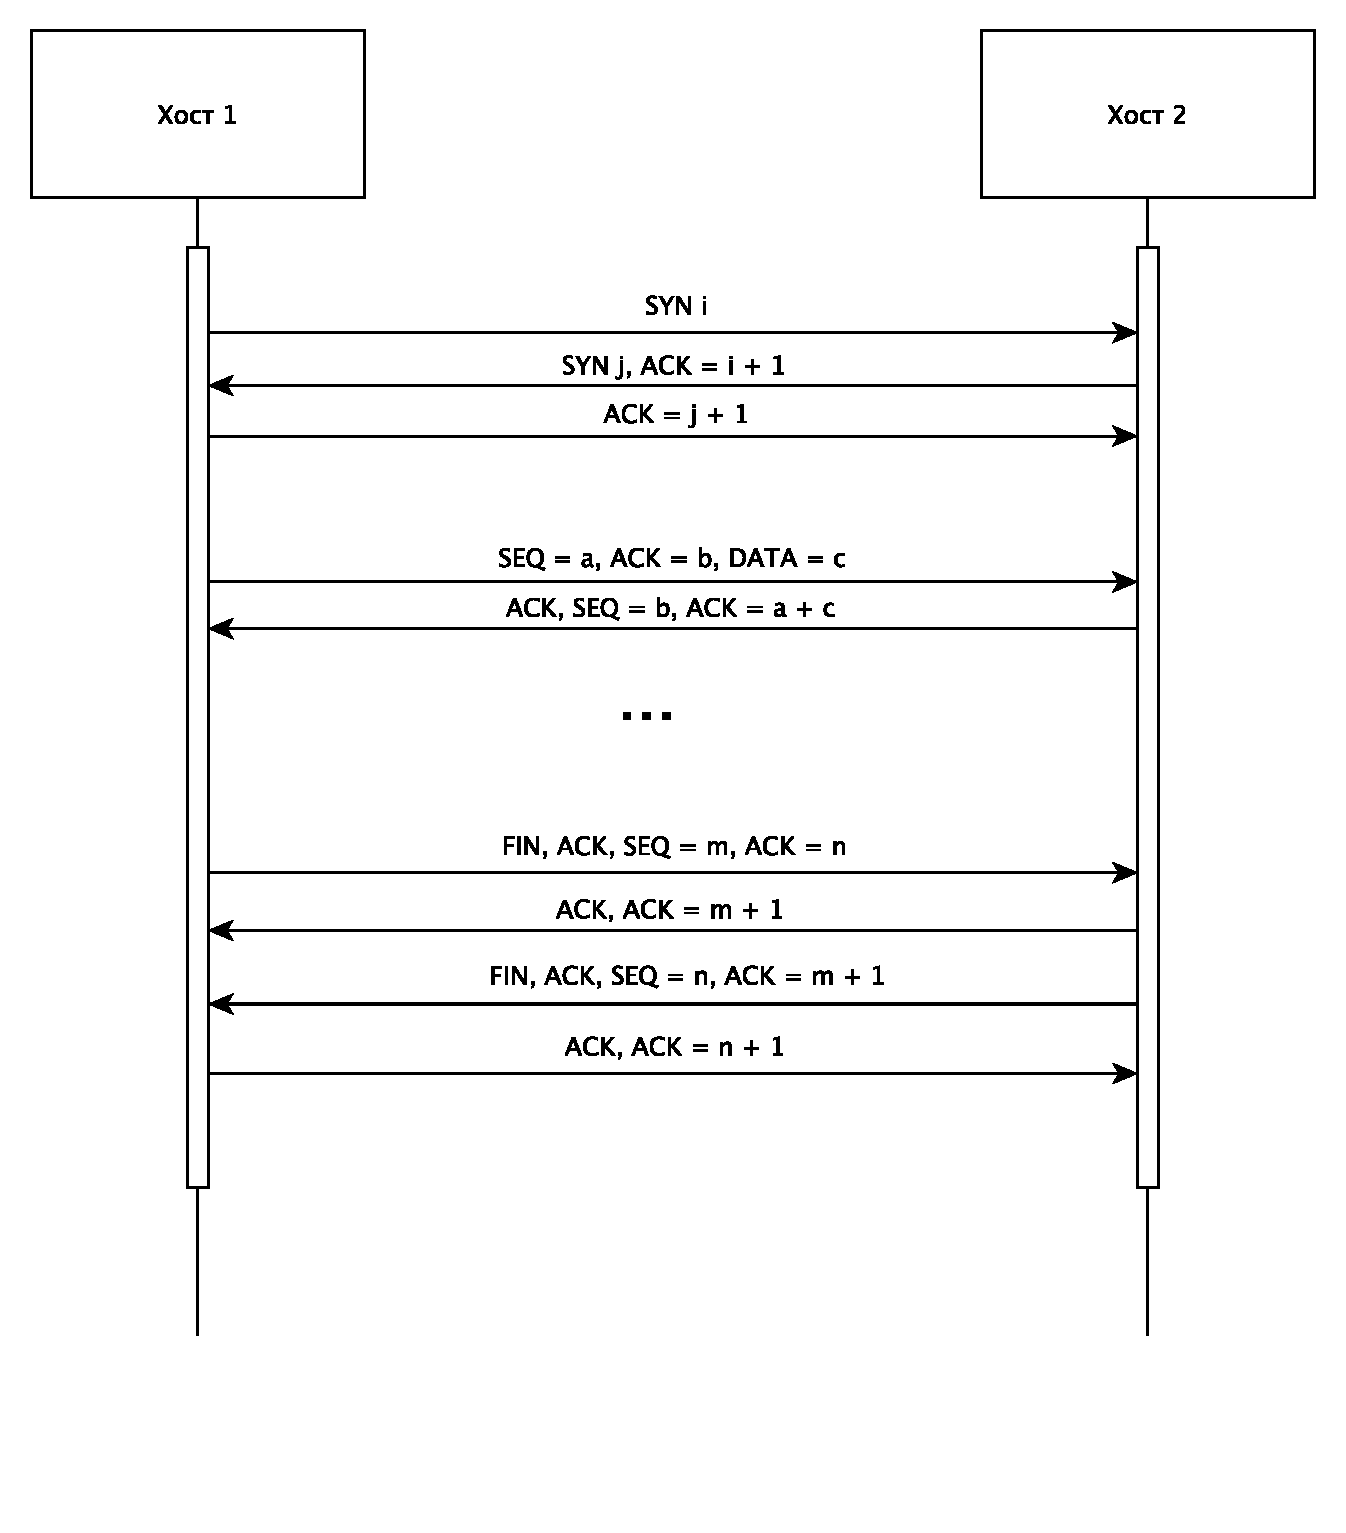
\includegraphics[width=\textwidth]{inc/1.pdf}
	\caption{ UML-sequence диаграмма взаимодействия двух хостов с использованием протокола TCP. }
	\label{img:1}
\end{figure}

\subsection{Описание модели и результаты}

Описание модели представлено в листинге \ref{lst:1}.

\begin{lstlisting}[label=lst:1,caption=Описание модели взаимодействия процессов.]
	#define MAX_BUF 2
	#define DATA_MESSAGES_COUNT 2
	
	mtype {DATA, ACK, SYN, SYN_ACK, FIN_ACK};
	
	chan client_to_server = [MAX_BUF] of {int, mtype};
	chan server_to_client = [MAX_BUF] of {int, mtype};
	
	proctype Client() {
		int data = 1337;
		int seq_num = 0;
		mtype msg_type;
		
		printf("Клиент отправляет SYN\n");
		client_to_server ! data, SYN;
		
		server_to_client ? _, msg_type;
		if
		:: (msg_type == SYN_ACK) ->
			printf("Клиент получает SYN-ACK от сервера и направляет в ответ ACK\n");
			client_to_server ! 0, ACK;
		fi
		 
		do
			:: seq_num < DATA_MESSAGES_COUNT ->
				printf("Клиент отправляет данные %d\n", data);
				seq_num++;
				msg_type = DATA;
				client_to_server ! data, DATA;
				data++;
				server_to_client ? _, msg_type;
				if
				:: (msg_type == ACK) ->
					printf("Клиент получает ACK от сервера\n");
				fi
			
			:: else ->
				break;
		od
			
		server_to_client ? _, msg_type;
		if
		:: (msg_type == ACK) ->
			printf("Клиент получает ACK от сервера\n");
		fi
	
		printf("Клиент направляет FIN_ACK серверу\n")
		client_to_server ! 0, FIN_ACK;
	
		server_to_client ? _, msg_type;
		if
		:: (msg_type == ACK) ->
			printf("Клиент получил ACK от сервера\n")
		fi
	
		server_to_client ? _, msg_type;
		if
		:: (msg_type == FIN_ACK) ->
			printf("Клиент получил FIN_ACK от сервера\n")
		fi
	
		printf("Клиент направляет последний ACK серверу и на этом заканчивает работу\n")
		client_to_server ! 0, ACK;
	}
	
	proctype Server() {
		int received_data;
		mtype msg_type;
		
		client_to_server ? _, msg_type;
		if
		:: (msg_type == SYN) ->
			printf("Сервер получает SYN от клиента и направляет в ответ SYN_ACK\n");
			server_to_client ! 0, SYN_ACK;
		fi
		
		client_to_server ? _, msg_type;
		if
		:: (msg_type == ACK) ->
			printf("Сервер получает ACK от клиента\n");
			server_to_client ! 0, ACK;
		fi
		
		printf("Сервер ожидает данные\n");
		client_to_server ? received_data, msg_type;
	
		do
			:: (msg_type == DATA) ->
				printf("Сервер получает данные %d и отправляет ACK в ответ клиенту\n", received_data);
				server_to_client ! 0, ACK;
				client_to_server ? received_data, msg_type;
	
			:: (msg_type == FIN_ACK) ->
				printf("Сервер получает FIN_ACK от клиента и направляет клиенту ACK и FIN_ACK\n")
				server_to_client ! 0, ACK;
				server_to_client ! 0, FIN_ACK;
				break;
		od
	
		client_to_server ? 0, msg_type;
	
		if
		:: (msg_type == ACK) ->
			printf("Сервер получил ACK от клиента и завершает работу\n")
		fi
	}
	
	init {
		atomic {
			run Client();
			run Server();
		}
	}
	
\end{lstlisting}

На рисунке \ref{img:2} представлены логи SPIN, демонстрирующие работу модели.

\begin{figure}[H]
	\centering
	\includegraphics[width=\textwidth]{inc/2.png}
	\caption{ Логи SPIN, демонстрирующие работу модели. }
	\label{img:2}
\end{figure}

\pagebreak